\section{The Block Tree Functionality}\label{sec.functionality}

We begin by noting that certain aspects of finite protocol executions cannot
apply in the infinite model. First, polynomially-bound executions indirectly
imply that the execution time of a party's round must be polynomial. However, in
the unbounded case there is no guarantee that the adversary will ever yield
control to the environment so that the execution of a round can continue. We
therefore must restrict our treatment to adversaries which, even though
unbounded and potentially never halting in an execution of infinite rounds, have
the property that \emph{each of their invocations in an individual round must
always eventually return control to the environment}. This ensures that the
protocol will make progress.

In typical proof-of-work blockchain treatments~\cite{EC:GarKiaLeo15}, the
probability $p$ of mining a block is achieved by modeling the block generation
process as a fresh query to a Random Oracle which returns a $\kappa$-bit
long string $H(B)$, where $\kappa$ is the security parameter and $B$ are the
candidate block contents. If the proof-of-work equation $H(B) \leq T$ holds, the
block is deemed \emph{successful} and each party is given $q$ such queries per
round. The probability of a query being successful is then calculated as $p =
\frac{T}{2^\kappa}$. The block contents $B$ contain a pointer to the previous
block in the chain. The security of such a scheme requires that there will be
no collisions in the output $H(B)$ such that every block can be uniquely
identified by its hash and the chain has no insertions or cycles. This can be
established with overwhelming probability in the polynomial case, but it is
insufficient for exponential executions. Clearly, if an execution is left to run
for an infinite amount of time, a collision within the finite-sized output space
$\{0, 1\}^\kappa$ will occur after at most $2^\kappa + 1$ queries. It follows
that the use of a security parameter cannot be applied in the unbounded case.

Instead, we put forth a functionality which captures the essential properties of
chains --- that the blocks will form a tree with no cycles, and that a party can
mine on top of a block only if they have first \emph{seen} it on the network.
One difficulty with this approach is that blocks can no longer be represented by
identifier strings which can be shared on the network, due to the reason
that an unbounded adversary could simply \emph{guess} that string if they have
a sufficient amount of time. Therefore, the functionality must maintain
knowledge of which blocks have been generated, which blocks extend which parent,
and which blocks are known to whom. Furthermore, the functionality must ensure
that the query limits are respected and that each query maintains a constant
probability of success $p$.

Instead of identifying each block by its hash, the functionality numbers blocks
sequentially and refers to them by their \emph{index}. Therefore, genesis is
referred to as $1$, the first block after genesis is referred to as $2$ and so
forth. The functionality maintains a map which keeps track of which parties are
aware of which blocks. This is useful as the adversary can withhold blocks and
it must not be possible to mine on top of them. The index of a specific block
may be different in the view of different parties, as blocks can be received in
a different order. When party $p_1$ refers to block with index $i$, it may be a
different block from the block with index $i$ referred by party $p_2$. The
block tree functionality maintains a \emph{global view} of the tree, while each
party has a \emph{local view} of the tree, with potentially different indices.
This is illustrated in Figure~\ref{fig:functionality-views}.

The full functionality is illustrated in Figures~\ref{fig:blocktree1}
and~\ref{fig:blocktree2}. All methods can be used by both the honest parties and
the adversary, with the exception of the method $\snoopmail$ and $\injectmail$
which highlights the network advantage of a \emph{rushing adversary} and can
only be used by her. Furthermore, honest parties always reveal by issuing a
$\broadcast$ and so a selective $\reveal$ will only be used by the adversary.

\import{./}{blocktree.tex}

\begin{figure*}
\begin{center}
    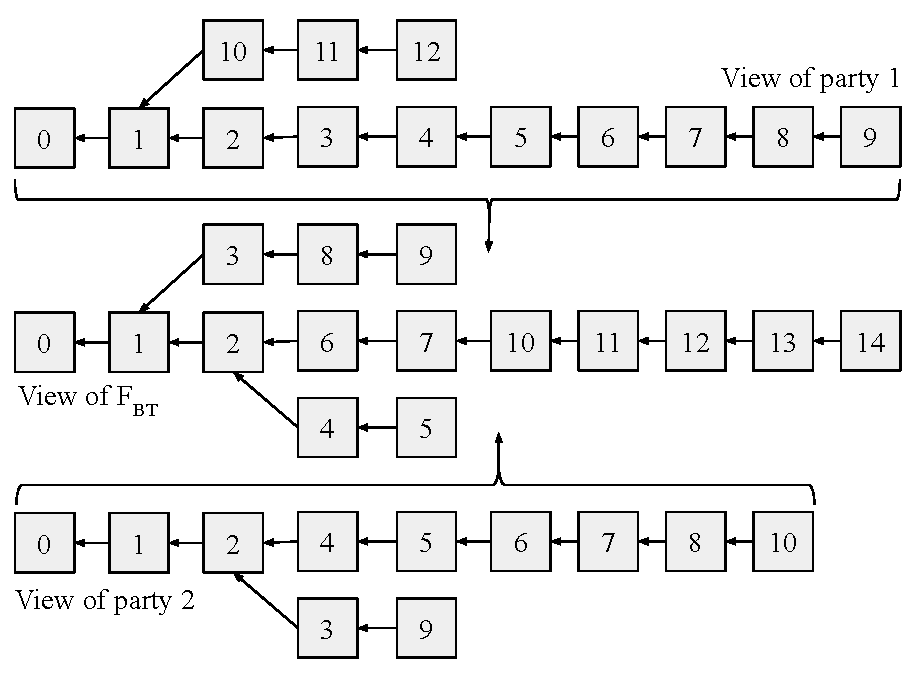
\includegraphics[width=0.8\textwidth]{fig/functionality-views.pdf}
  \caption{The global view of the blocktree functionality is the combined view
  of partial local views of individual parties.}
  \label{fig:functionality-views}
  \end{center}
\end{figure*}

\begin{remark}[Globally indexed blocks]
We could have opted to simply index blocks by the global order of generation and
every party could use the same index to refer to the same block, as the
functionality is aware of all queries. This would simplify the treatment, but it
would open up the possibility for a party to determine whether another party is
withholding a block by looking at this global counter, a behavior which does not
correspond to the way the real protocol works. The cryptographic treatment which
we follow in this paper mandates that there is \emph{one} adversary and the rest
of the parties are honest, and so this does not make a difference; however, it
does make a difference in treatments in which the incentives of the parties are
analyzed (c.f.~\cite{C:KRDO17}) and there are multiple non-cooperating parties
% TODO: cite Stouka
which can deviate from the honest protocol. We therefore insist on the detail
that each party can have a different view for the index of each block.
\end{remark}

\begin{remark}[Polynomial-time block trees]
While here the block tree functionality is conjured as
\emph{deus ex machina} and cannot be implemented in practice for infinite
executions, it captures and encapsulates the essential combinatorial properties
desired in blockchain protocols. As such, it can also be used in the polymomial
setting as an encapsulation mechanism to achieve proof modularity: First,
it can be shown that some implementation technique (for example, the Random
Oracle model together with the proof-of-work equation $H(B) \leq T$) is
sufficient to provide the functionality's properties with overwhelming
probability; second, the functionality can be treated as \emph{black box} and it
can be shown that the blockchain protocol works as desired given the
functionality's properties. While the first proofs are probabilistic, the latter
are combinatorial. In fact, while this intermediate functionality is not
presented explicitly in previous works, the separation of the probabilistic and
combinatorial proofs appeared in the context of a \emph{typical execution}
in~\cite{EC:GarKiaLeo15}, although the treatment is not black box.
% TODO: Cite Pass here?
\end{remark}
